In Chapter \ref{ch:functor_languages} we presented an implementation of the semantics of Casanova by using the language extension of Metacasanova with functors and modules. This new implementation improved the performance of the language re-implemented in Metacasanova of 42 times with respect to the previous implementation described in Chapter \ref{ch:languages}. In this chapter we further extend Casanova with language primitives to describe the network mechanism for an online multiplayer game. We start this chapter by introducing the problem of developing an online multiplayer game and the existing approaches. We then propose a language extension for Casanova to integrate primitives to support network data synchronization that should aid the developer of online multiplayer games, which has also been presented in \cite{DIGIACOMO201725}\footnote{The work described in this Chapter was realised in cooperation with Mohamed Abbadi and a preliminary version appears also in the appendix of his thesis. The content of Sections \ref{sec:ch_networking_mpsupport} to \ref{sec:ch_networking_casanova_networking_primitives} thus appears also in the appendix of \cite{abbadithesis2017} and in the paper \cite{DIGIACOMO201725}}. We then show that the new implementation of Casanova in Metacasanova presented in Chapter \ref{ch:functor_languages} can be extended to include the new networking semantics. In the result we analyse the performance of Casanova with the networking extension when compiled by its hard-coded compiler in F\# with respect to the same sample implemented in C\#. Moreover we compare the effort in terms of lines of codes necessary to implement the network semantics in the hard-coded version of the compiler and in Metacasanova.

\section{Multi-player Support in Games}
\label{sec:ch_networking_mpsupport}
Adding multi-player support to games is a highly desirable feature. By letting players interact with each other, new forms of gameplay, cooperation, and competition emerge without requiring any additional design of game mechanics \cite{granberg2014david}. This allows a game to remain fresh and playable, even after the single player content has been exhausted. For example, consider any modern AAA (AAA refers to games with the highest development budgets\cite{wolf2008video}) game such as \textit{Halo 4}. Within months after its initial release, most players have exhausted the single player, narrative-driven campaign. Nevertheless the game remains heavily in use thanks to multiplayer modes, which in effect extended the life of the game significantly. This phenomenon is even more evident in games such as \textit{World of Warcraft} or \textit{EVE}, where multiplayer is the only modality of play and there is no single-player experience.

\paragraph{Challenges}
Multi-player support in games is a very expensive piece of software to build. Multiplayer games are under strong pressure to have very good \textit{performance} \cite{claypool2006latency}. Performance is both expressed in terms of CPU time and in bandwidth used. Also, games need to be very \textit{robust} with respect to transmission delays, packets lost, or even clients disconnected. To make matters worse, players often behave erratically. It is widespread practice among players to leave a competitive game as soon as their defeat is apparent (a phenomenon so common to even have its own name: ``rage quitting'' \cite{rage_quitting}), or to try to abuse the game and its technical flaws to gain advantages or to disrupt the experience of others.

Networking code reuse is quite low across titles and projects. This stems from the fact that the requirements of every game vary significantly: from turn-based games that only need to synchronize the game world every few seconds, and where latency is not a big issue, to first-person-shooter games where prediction mechanisms are needed to ensure the smooth movement of synchronized entities, to real-time strategy games where thousands of units on the screen all need to be synchronized across game instances \cite{smed2002aspects}. In short, previous effort is substantially inaccessible for new titles. 

Encapsulation suffers from this ad-hoc nature of the implementation of the networking layer in multiplayer games. Indeed managing the information about game updates over a network requires each game entity to interface the game logic code with network connection and socket objects, data transmission method calls such as ``send'' and ``receive'', and support data structures to manage traffic and track the status of common protocols. This happens because each game entity must provide the following functionality in order to work in a multiplayer game:

\begin{itemize}
	\item Update the logic in the fashion of a singleplayer counterpart.
	\item Choose what data is necessary to send over the network and create the message containing this information.
	\item Choose what data can be lost and what data must always be received by the other clients.
	\item Periodically check if incoming messages contain information that needs to be read and to perform specific updates.
\end{itemize}

Combining these requirements together within the same entity breaks encapsulation because the entity's logic gets mixed with spurious details of the networking implementation. Maintenance then becomes very hard, as every change in the game logic must also be reflected in the networking implementation.

\paragraph{Existing approaches}
Networking in games is usually built with either very low-level or very high-level mechanisms. Very low-level mechanisms are based on manually sending streams of bytes and serializing only the essential bits of the game world, usually incrementally, on unreliable channels (UDP). This coding process is highly expensive because of the difficulties of manually implementing such a low-level protocol. Debugging subtle protocol mismatches, transmission errors, etc. will take lots of development resources. Low-level mechanisms must also be very robust, making the task even harder.

An alternate approach is to use high-level protocols such as RDP, reflection-based serialization, frameworks (such as Pastry, netty.io), etc. can also be used. These methods greatly simplify networking code, but are rarely used in complex games and scenarios. The requirements of performance mean that many high-level protocols or mechanisms provide insufficient efficiency, either because they are too slow computationally (especially when they rely on reflection or events) or because they transmit too much data across the network.

\section{Motivation for a Language-based Solution}

To avoid the problems of both existing approaches, we propose a middle ground. We observe that networking fundamental abstractions upon which the actual code and protocols are built do not vary substantially between games, even though the code that needs to be written to implement them does. The similarity comes from the fact that the ways to serialize, synchronize, and predict the behaviour of entities are relatively standard and described according to a limited series of general ideas. The difference, on the other hand, stems from the fact that low-level protocols need to be adapted to the specific structure of the game world and the data structures that make it up. Until now, common primitives have not been syntactically and semantically captured inside existing domain-specific languages for game development \cite{bhatti2009domain}. Using the right level of abstraction, these general patterns of networking can be captured, while leaving full customization power in the hand of the developer (to apply such primitives to any kind of game).

\section{Related work}
In the following we discuss some existing networking tools used in game development and we highlight some issues that arise from their use.

\paragraph{The Real time framework (RTF)} RTF \cite{glinka2007rtf} is a middleware built for C++ to relieve the programmer from dealing with data compression. It is more flexible than solutions based on game engines or hand-made implementations, since it automates the process of data transmission. Moreover, it supports distributed server management. Unfortunately, this solution has several flaws:
\begin{itemize}
	\item All entities must inherit from the class \texttt{Local} and the semantics of the position is pre-determined, often clashing with rendering or physics.
	\item Platform independence requires that the programmer uses RTF primitive	types.
	\item Data transmission automation requires that all game entities inherit the class \texttt{Serializable}.
	\item Being a middleware, RTF is not aware of what games are going to use it for (every game comes with different data structures). Thus, the developer is tasked to include in his code also logic to update the RTF layer, in order to keep the game updated over the network.
\end{itemize}


\paragraph{Network scripting language (NSL)} NSL \cite{russell2008tackling} provides a language extension based on a send-receive mechanism. Moreover it provides a built-in client side prediction (a feature missing in existing highly concurrent and distributed languages such as Stackless Python \cite{kalogirou2005multithreaded} and Erlang \cite{armstrong1993concurrent}), which is periodically corrected by the server. 

\paragraph{Unreal Engine/Unity Engine} Unreal Engine \cite{games2006unreal} and Unity Engine \cite{engine9unity} are commercial game engines supporting networking.  Both Unity and Unreal Engine use a client-server approach. In Unreal Engine, the server contains the ``true'' game state, and the clients contain a ``dirty'' copy, which is validated periodically. It is possible to define entities (actors in Unreal Engine jargon) that are replicated on the clients. Whenever a replicated actor changes on the server, this change is also reflected on the clients. Additional customization can be achieved through Remote procedure calls (RPCs) of three kinds.
\begin{itemize}
	\item The function is called on the server and executed on the client. This is used for game elements that do not affect gameplay, such as creating a particle effect when a weapon is fired.
	\item The function is called on the client and executed on the server. This is useful for events that affect the other clients and should be validated by the server.
	\item The function is executed in multi-cast, meaning that the server calls the function and that it is executed on both the server and all the clients.
\end{itemize}

The Unity Engine uses a similar approach based on networking components, synchronized at every frame, and RPC's to define custom synchronization events.

Unfortunately, customization comes at the cost of the level of detail that developers must face. Using RPC's require a deep knowledge of the engine and writing lots of code. 

In this section we introduce a small example that addresses the requirements of designing a multiplayer game. We then present an architecture that aims to fulfil these requirements.

\section{The master/slave network architecture}

We chose to implement the networking layer in Casanova by using a peer-to-peer architecture for the following reasons:

\begin{itemize}
	\item Server-client architectures are more reliable but suitable only for specific genres of games (mostly Shooter games), while other genres, such as Real-time strategy games and Online Role Playing Games, use P2P architectures.
	\item By using a P2P architecture, we do not have to write a separate logic for an authoritative game server, which has to validate the actions of clients.
\end{itemize}

Casanova will provide a generic tracking server, which is run separately from the main program. The tracking server is a thin service that connects players participating in a single game, and helps with forwarding the network traffic through NATs (Network Address Translation).

Each client maintains a local copy of the \texttt{world} entity and has direct control over a single portion of it. Instances belonging to such as portion are seen as \textit{master} by this client, who is always allowed to directly change the state of the master instances without having to validate this state change by synchronizing with other clients through the network.

Each client also maintains a portion of the world that is not directly under his control. Instances belonging to such as portion are seen as \textit{slave} by this client, who is only allowed to \textit{predict} the local state of the instances and, whenever he receives an update from their masters, must correct this prediction according to the data contained in the received messages. The slave part of the world is thus maintained passively by the client: the only active part is predicting the evolution of the entity dynamics and correcting it whenever it receives an update by its master.

For this purpose, we extend the syntax of Casanova rules by allowing them to be marked with the modifiers \texttt{master} and \texttt{slave}. These rules are executed respectively on master and slave entities. Note that it is still possible not to mark a rule with these modifiers, which means that the rule is always executed independently of the fact that the entity is either master or slave on that particular client. We also allow to mark a rule as \texttt{connecting} and \texttt{connected}. These rules are triggered only once respectively when a new client connects and when the clients detect a new connection.

Casanova also provides primitives to send (reliably or unreliably) and receive data. A schematic representation of this architecture can be seen in Figure \ref{fig:masterslave}.

\begin{figure}[h!]
	\centering
	\caption{Representation of the game world in a networking scenario}
	\label{fig:network_world}
	\begin{subfigure}[t]{0.3\linewidth}
		\centering
		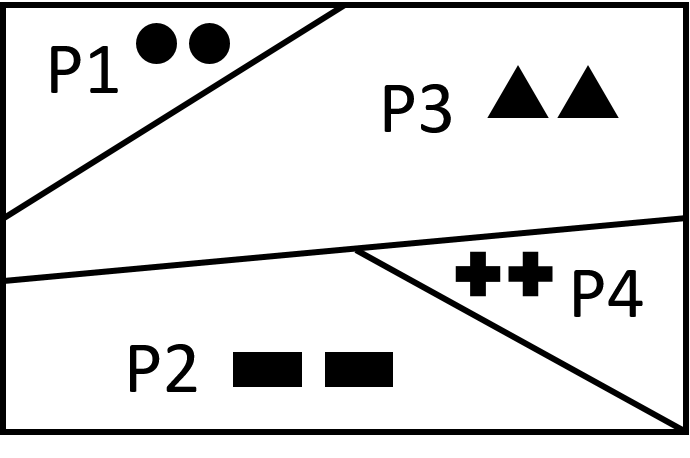
\includegraphics[width=1\linewidth]{Figures/networking2}
		\caption{Unknown correct game state when P3 joins the game.\\}
		\label{subfig:networking_ideal}
	\end{subfigure}
	\begin{subfigure}[t]{0.3\linewidth}
		\centering
		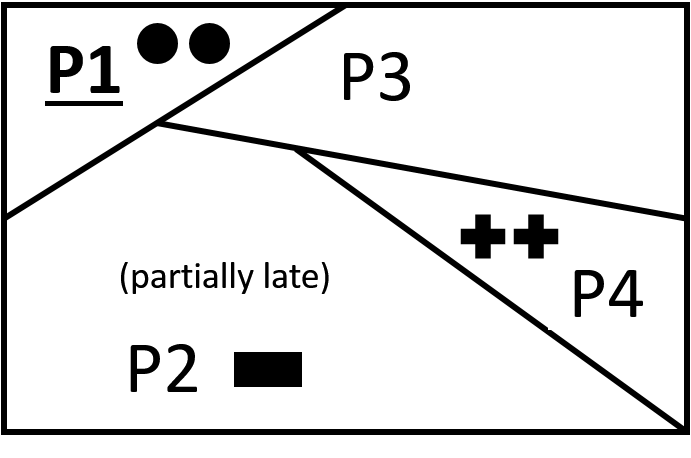
\includegraphics[width=1\linewidth]{Figures/networking1}
		\caption{Networking game state seen from the point of view of P1. P2 is partially synchronized, P4 is fully synchronized, and P3 is a new client that is late and is still sending its data}
		\label{subfig:networking_relative}
	\end{subfigure}
	
	
\end{figure}

\begin{figure}
	\centering
	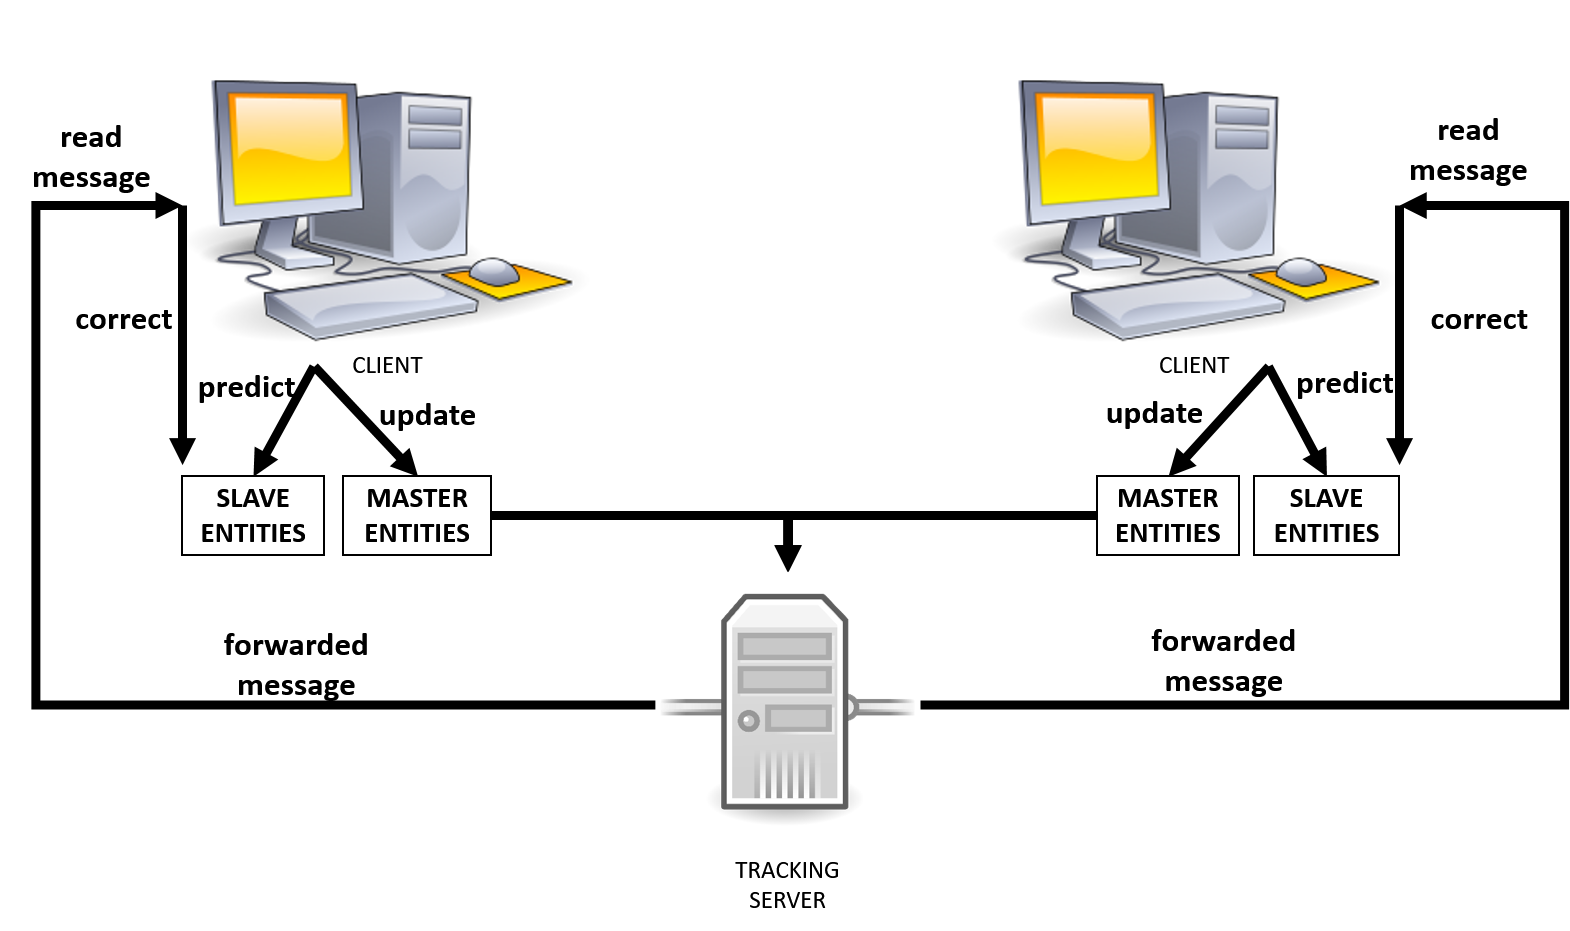
\includegraphics[width = \textwidth]{Figures/masterslave}
	\caption{master/slave architecture}
	\label{fig:masterslave}
\end{figure}

Note that the aim of this architecture is to provide language-level primitives to describe the networking logic. This means that the compiler will be able to generate code compatible with the low-level network libraries that provide transmission functions over the network channel without having to change Casanova code in the program. In our implementation, we chose the .NET library \texttt{Lidgren}, which is widely used also in commercial game engines such as Unity3D and MonoGame, but nothing prevents the compiler to be expanded in order to target other similar libraries for other languages, such as jgroups \cite{ban2002jgroups}.

\section{Case study}
Let us consider a simple shooter game where each player controls a space ship. Players can move forward, backward, and rotate the ship to change direction. Moreover, they can use the ship lasers to shoot other players. If a laser hits an enemy ship, we increase the player's score. Designing such a game requires to address the following issues, depicted by the schematic representation in Figure \ref{fig:network_world}:

\begin{enumerate}
	\item Each player must maintain a local version of the game state (world). In order to avoid to flood the network with messages, all the copies are not fully synchronized at each frame, thus they are slightly different and each client knows the latest version of only part of the copy.
	\item A player \texttt{connecting} to an existing game must be able to receive the latest update of the game state and send the new ship he will control to existing players in the game.
	\item A player already \texttt{connected} to the game must detect a new connection and send his master portion of the game state.
	\item Each player must be able to control only one ship at a time. This means that the part of the game logic that processes the input and modifies the spatial data of the ship (position and rotation) should only be executed on the ship controlled by the player and not on the local copies of other players' ships. This means that each player sees as \texttt{master} only one ship instance.
	\item Each player must send the updated state of the ship he controls to the other players after executing the local update. To achieve better performance over the network, the data is not sent at every update, but with a lower frequency.
	\item Each player must receive the updated state of \texttt{slave} ships controlled by other players. In this phase, we must take into account that, as explained above, not every update is sent, so the player should ``predict'' what will happen during the game frames in which he does not receive an update.
\end{enumerate}

\section{Implementation}
\label{sec:ch_networking_casanova_networking_primitives}
Each of the scenarios described above requires specific language extensions. These extensions identify connection, ownership (master/slave), and various send and receive primitives. In this section, we introduce each primitive by using a multiplayer game example. We now give an implementation of the shooter game presented above, using the extended version of Casanova with network primitives. The \texttt{world} contains a list of ships controlled by each player.
\begin{lstlisting}
world Shooter = {
  Ships  : [Ship]
  ...
}
\end{lstlisting}

Each \texttt{Ship} contains a position, a rotation, a collection of shot projectiles, and the score.
\begin{lstlisting}
entity Ship = {
  Position   : Vector2
  Rotation   : float32
  Projectiles : [Projectile]
  Score		  : int
  ...
}

\end{lstlisting}

Each \texttt{Projectile} contains its position and velocity.

\begin{lstlisting}
entity Projectile = {
  Position : Vector2
  Velocity : Vector2
  ...
}
\end{lstlisting}

\subsubsection{Connection}
When a player connects, we must consider two different situations: (\textit{i}) a player is already in the game and must send the current game state to the connecting players, and (\textit{ii}) the player who is connecting needs to send the ship he will instantiate and control (its initial state). Both the players in the game and the connecting one must receive the game states that are sent. For this purpose we introduce two additional modifiers, \texttt{connecting} and \texttt{connected}, that can be added to rule declarations to mark their role in the multiplayer logic.

\paragraph{Connecting} A rule marked with \texttt{connecting} is executed once when a player joins the game for the first time. In our example, the player should send his initial state (the created ship) to the other players. We use the primitive \texttt{send\_reliable} because we must be sure that eventually all players will be notified of the ship creation.
\begin{lstlisting}
world Shooter = {
  ...
  rule connecting Ships =
  yield send_reliable Ships
}
\end{lstlisting}

\paragraph{Connected} A rule marked with \texttt{connected} is run whenever a new player joins the game by all existing players. When this occurs, each player sends its ship. The system will take care to send only the ship controlled locally by the player itself for each player. The rule will use the \texttt{send\_reliable} primitive for the same reason explained in the previous point.

\begin{lstlisting}
world Shooter = {
  ...
  rule connected Ships =
  yield send_reliable Ships
}
\end{lstlisting}

Note that even if the code is the same, the semantics of the two rules are different. The first one is executed by the player joining the game, who locally instantiates its \texttt{Ship} and must send its list of \texttt{Ships} (containing only the local instance) to the other players. The second one is executed by all existing players who must share with the joining player the list of existing ships.


\subsubsection{Master updates}
As explained above, each client manages a series of local game objects (called \textit{master objects}) that are under its direct control. The other clients read passively any update done on those instances and update their remote copy  (\textit{slave objects}) accordingly. We mark rules affecting the behaviour of master objects as \texttt{master}. In our example, the following situations are run as master: (\textit{i}) synchronizing the ships among players, (\textit{ii}) updating the ship and projectiles spatial data, and (\textit{iii}) creating and destroying projectiles.

\begin{enumerate}
	\item Each player is tasked to maintain the list of Ships in the world. This requires to receive the updated list from other players and to store the new value in a master rule. Indeed the world is a special case of an entity that is shared among players, and not directly owned by somebody. Each ship contained in that list and received from other players will be treated appropriately as slaves, while the only one owned by the current player will be under his direct control. In this rule we use \texttt{let!}, which is an operator that waits until the argument expression returns a result and then binds it to the variable. The symbol \texttt{@} stands for list concatenation. The rule uses \texttt{receive\_many}, which receives and collects the list of sent ships by the other players.
	
	\begin{lstlisting}
	world Shooter = {
  	...
  	rule master Ships =
  	let! ships = receive_many()
  	yield Ships @ ships
	}
	\end{lstlisting}
	
	\item The master version of the ship update reads the input of the player and moves (or rotates) the ship if the appropriate key is pressed. Note that this part must be executed only on a master object, because we want to allow each player to control only the ship he owns and instantiates at the beginning of the game. Below we show just the rule to move forward; the other movement and rotation rules are analogous. We use an \textit{unreliable send} (in the code we are using \texttt{send} and not \texttt{send\tu reliable} as done previously) because it is acceptable to lose an update of the position during a certain frame: shortly after, there will be a new update. Casanova allows the programmer to choose whether to use reliable or unreliable transmissions in the code.
	
	\begin{lstlisting}
	entity Ship = {
	...
	rule master Position =
  	wait world.Input.IsKeyDown(Keys.W)
  	let vp = new Vector2(Math.Cos(Rotation), 
  	Math.Sin(Rotation)) * 300.0f
  	let p = Position + vp * dt
  	yield send p
	}
	\end{lstlisting}
	
	We do the same for projectiles, except the projectile position is continuously updated and synchronized over the network without having to wait that a key is pressed.
	
	\item Creating a new projectile happens when the player shoots. A ship keeps track of the projectiles it has shot so far, and adds a new one to the list of the existing projectiles. The updated list is sent to all players with the new instance of the projectile (which is added as a new head of the list with the operator \texttt{::}). Here it is better to specify the semantics of the \texttt{yield} in conjunction with the use of networking primitives. A \texttt{yield} requires that the written value is type-compatible with the domain of the rule. Thus, when used with a \texttt{send} primitive, we must pass a list as argument. The system will ensure, for performance reasons, that the generated code only sends items which are newly added to the list. These semantics are defined like this for two main reasons: (\textit{i}) when sending the new projectiles we must also update the list in local (and given the immutability of Casanova we must replace the existing one), and (\textit{ii}) because in this way the programmer can focus on the logic of the game as if it were a single-player game without worrying of network-specific details. Note that the last \texttt{wait} forces the player to release the key before shooting again (semi-automatic fire). Removing that check would spawn multiple projectiles consecutively, which is not a wanted behaviour.
	
	\begin{lstlisting}
	entity Ship = {
	...
	rule master Projectiles =
	wait world.Input.IsKeyDown(Keys.Space)
	let vp = new Vector2(Math.Cos(Rotation), 
	Math.Sin(Rotation)) * 500.0f
	let projs = new Projectile(Position, vp) :: Projectiles
	yield send_reliable projs
	wait not world.Input.IsKeyDown(Keys.Space)
	}
	\end{lstlisting}
	
	Filtering the colliding projectiles and updating the score is run as a master rule. The rule computes the set difference between the ship projectiles and the colliding projectiles and updates the list of projectiles, sending them through the network as well. Even in this case, the network layer sends only the information about the projectiles to remove. Note that the score is managed by each player locally, as it does not require to be synchronized (we do not print the other players' scores. Doing so would indeed require to also send the score).
	
	\begin{lstlisting}
	entity Ship = {
	...
	rule master Projectiles, Score =
  	let collidingProjs =
  	 [for p in Projectiles do
  	   let ships =
  	     [for s in Ships do
  	       where 
	           s <> this and 
  	         Vector2.Distance(p.Position,s.Position) < 100.0f
  	       select s]
  	 where ships.Count > 0
  	 select p]
  	let newProjectiles = Projectiles - collidingProjs
  	yield send_reliable newProjectiles, 
  	Score + collidingProjs.Count 
	}
	\end{lstlisting}
\end{enumerate}

\subsubsection{Managing remote instances}
The game objects that were not instantiated by a client, but received from another client, are \textit{slave objects} and must be synchronized differently than master objects. For this purpose, a rule can be marked as \texttt{slave}. In our example, we use slave rules in the following situations: (\textit{i}) synchronizing other players' ships and projectiles spatial data, and (\textit{ii}) projectiles instantiated by other players.

\begin{enumerate}
	\item Every remote projectile and ship is synchronized locally by a rule, which tries to \texttt{receive} a message containing updated spatial data. Below we provide the code to update the position of the ship; the synchronization of other spatial data is analogous.
	
	\begin{lstlisting}
	entity Ship = {
	 ...
	 rule slave Position = yield receive()
	}
	\end{lstlisting}
	
	\item When a projectile is instantiated remotely, we have to receive it and add it to the list of projectiles. We use \texttt{receive\_many} because the new projectiles are added to a list. This case also supports the situation where a ship could shoot multiple projectiles at the same time.
	
	\begin{lstlisting}
	entity Ship = {
	 ...
	 rule slave Projectiles =
	 let! projs = receive_many()
	 yield projs @ Projectiles
	}
	\end{lstlisting}
\end{enumerate}

In this scenario we have to discuss the atomicity of these transmissions: in the context of network games, reliability is often sacrificed for better network performance, so most of the data transmissions are unreliable (like in the case of the ship position). This means that we have no guarantee that the message will be received. Several issues can arise from this situation: for example, if a client fails to receive the position of the ship, then it might miss a collision with a projectile. Out-of-sync errors might happen during a multiplayer game, and their effect is a well-known issue in several shooter games where players affected by high latency or packet loss see in their view of the game a hit on the player when this is not seen by the other players who did not receive the information regarding this event. Ensuring that all the data transmissions are reliable might on the other hand affect network performance to the point that the game would become unplayable because of the network overload. 

Casanova allows the programmer to decide whether the transmission should be reliable or not and experiment with the effect of a reliable transmission versus an unreliable one that does not overload the network. For example, the updated list of projectiles, after a collision, is always sent in a reliable way. This is acceptable because collisions are not so frequent. This is not true for the ship position, since movements are very frequent and mostly happen at every frame, thus it is something that is not necessary to be sent reliably at every frame.

\section{Networking Primitives with Functors}
\label{sec:ch_networking_functor_networking}
In the Chapter \ref{ch:functor_languages} we described in detail how to implement the logic of the Casanova update traversal with functors in Metacasanova. We also further extended its first implementation with interruptible rules. In this section we show a sketch of how to use functors to implement the networking primitives introduced in Casanova in Section \ref{sec:ch_networking_casanova_networking_primitives}. In what follows we assume that the data transfer primitives are defined in an external library that we assume it is given, since the same applies to the implementation presented in Section \ref{sec:ch_networking_casanova_networking_primitives}, and the send and receive primitives simply generate calls to this library.

\subsection{Network Record}
\label{subsec:ch_networking_network_record}
In order to implement the logic of master/slave entities we need to store additional information in a Casanova entity to know if its instance has been created locally (thus being master). At this purpose we use a functor \texttt{NetworkRecord} to create an instance of a record module to store this information. This functor takes as input a record representing a Casanova entity and builds a new record instance by adding a boolean field used to store the ownership status.

\begin{lstlisting}
Functor "NetworkRecord" => Record : Record 

RecordField "__isLocal" bool r => r'
--------------------------------------
NetworkRecord r => networkRecord
\end{lstlisting}

\subsection{Connection}
\label{subsec:ch_networking_connection}
In order to implement the semantics of a connecting rule we have to modify the field (we rely on the implementation with the record seen in Figure \ref{fig:ch_networking_interruptible_rules}) to store not only the rule continuation but also its connection state. Note that, with this change, we have to change the return type of \texttt{tick} as well, because now the field is a triplet and not a pair. We also define a functor \texttt{ConnectingCoroutine} that instantiate a field updater sharing the same implementation that we generate from a normal coroutine, except for the logic of the function \texttt{update}. 

\begin{lstlisting}
Functor "ConnectingCoroutine" => string => Record => Record => string => stmt : FieldUpdater
\end{lstlisting}

\noindent
This time \texttt{update} has three evaluation rules. The first one creates a getter to retrieve the current field. It then calls the getter generated at the previous step to read the value of the connection status stored in the field. The following clause performs a check on the connection status. If the value is true then the clause fails and thus the rest of the premises is not executed because the whole evaluation rule fails and we skip to the next evaluation rule. If the value is false then we run the code of the rule. At this point if the continuation after the rule update is empty then the connecting rule has terminated its execution and we set to \texttt{true} the connection status. 

\begin{lstlisting}
----------------------------------
ConnectingCoroutine ruleName continuation r field stmts => FieldUpdater r field {
  ...
  
  
  GetField r field => getter
  GetField continuation ruleName => contGetter
  getter.get entity -> (v,(connected,cont))
  connected = false
  tick entity k dt -> (v',(c',k'))
  contGetter.get k' -> nop
  --------------------------
  update entity dt -> (v',(true,k'))
  
  ...
}
\end{lstlisting}

\noindent
The second evaluation rule differs from the first only in the fact that it is executed when the Casanova rule returns a non-empty continuation. In this case we do not set the connection status to \texttt{true} because the connecting rule has not terminated its execution yet.

\begin{lstlisting}
----------------------------------
ConnectingCoroutine ruleName continuation r field stmts => FieldUpdater r field {
  ...
  
  
  GetField r field => getter
  GetField continuation ruleName => contGetter
  getter.get entity -> (v,(connected,cont))
  connected = false
  tick entity k dt -> (v',(c',k'))
  --------------------------
  update entity dt -> (v',(c',k'))
  
  ...
}
\end{lstlisting}

\noindent
The third and final case of the evaluation rule is when the connection status has already been set to \texttt{true}; this means that the Casanova rule has already been evaluated completely during a previous update and does not need to be executed again.\\

\begin{lstlisting}
----------------------------------
ConnectingCoroutine ruleName continuation r field stmts => FieldUpdater r field {
  ...
  

  GetField r field => getter
  getter.get entity -> (v,(connected,continuation))
  connected = true
  getter.get entity -> (v,k)
  ------------------------
  update entity dt -> (v,k)
  
  ...

} 
\end{lstlisting}

\noindent
In the case of a connected rule, we need to be able to detect a new connection. This can be done in different ways: one possible solution is that when a client sends its data during the \texttt{connecting} phase, it sends also information about the connection. This step is handled at low level by the connection primitives. A Casanova rule marked as \texttt{connected} starts with a \texttt{wait} statement that checks if a new client has connected to the system. For the remaining part the rule behaves like a normal coroutine. Of course when the rule body has been completely evaluated, then it stops again until a new client connects, since the whole body will be reconstructed and thus also the \texttt{wait} statement

\subsection{Local and Remote Entities}
\label{subsec:ch_networking_local_and_remote}
The behaviour of master and slave rules can be modelled through dedicated functors that generate different instances for the field updater, in the same fashion as the \texttt{connecting} rule. We thus define two new functors \texttt{MasterCoroutine} and \texttt{SlaveCoroutine}. \texttt{MasterCoroutine} generates a field updater that has two different evaluation rules for \texttt{update}. The first one builds a getter for the field \texttt{\tu\tu isLocal}. It then uses it to read its value from the current entity and uses a clause to check whether the entity is local. At this point, if the entity is not local, the whole evaluation rule fails and the next one is run. Otherwise the Casanova rule body is run and the field updated accordingly to its specific code.

\begin{lstlisting}
Functor "MasterCoroutine" => string => Record => Record => string => stmt : FieldUpdater

----------------------------------------
 MasterCoroutine ruleName continuation r field stmts => FieldUpdater r field {
   ...
   
   GetField r "__isLocal" => localGetter
   localGetter.get entity -> (isLocal,(c,k))
   isLocal = true
   tick entity k dt -> (v',(c',k'))
   ------------------------------
   update entity dt -> (v',(c',k'))
   
   ...
\end{lstlisting}

\noindent
The second evaluation rule is used when the entity is not local. In this case the semantics of a \texttt{master} rule is simply not to be executed. In order to emulate this behaviour we simply return the content of the field as it is (including all the information on the Casanova rule state).
\begin{lstlisting}
----------------------------------------
 MasterCoroutine ruleName continuation r field stmts => FieldUpdater r field {
   ...
   
   GetField r "__isLocal" => localGetter
   GetField r field => getter
   localGetter.get entity -> (isLocal,(c,k))
   isLocal = false
   getter.get entity -> (v,(c,k))
   ------------------------------
   update entity dt -> (v,(c,k))
   
   ...
 }
\end{lstlisting}

\noindent
The \texttt{SlaveCoroutine} functor behaves in an analogous way: it generates two evaluation rules for \texttt{update} that are complementary to those of the \texttt{MasterCoroutine}. In this case the Casanova rule is updated only if the field \texttt{\tu\tu isLocal} is false. If this is not the case the second evaluation rule is triggered and it returns simply the field as it is.

\begin{lstlisting}
----------------------------------------
 SlaveCoroutine ruleName continuation r field stmts => FieldUpdater r field {
   ...

   GetField r "__isLocal" => localGetter
   localGetter.get entity -> (isLocal,(c,k))
   isLocal = false
   tick entity k dt -> (v',(c',k'))
   ------------------------------
   update entity dt -> (v',(c',k'))

   GetField r "__isLocal" => localGetter
   GetField r field => getter
   localGetter.get entity -> (isLocal,(c,k))
   isLocal = true
   getter.get entity -> (v,(c,k))
   ------------------------------
   update entity dt -> (v,(c,k))
   
   ... 
 }
\end{lstlisting}

\noindent
As a final note we want to point out that, since now the semantics of Casanova are encapsulated into the \texttt{FieldUpdater} instance generated by the \texttt{Coroutine} functor, by introducing different kinds of functors able to build the field updaters for coroutines we would need to duplicate the code of the semantics in the field updater modules instantiated by each functor. This is, of course, not a good a practice and the issue can be circumvented by creating an additional module, which we can call \texttt{CasanovaSemantics}, that contains the semantics of all the statements of Casanova. This module is instantiated in each field updater for coroutines by an utility functor defined internally to each field updater. When we need to refer to the semantics of a specific Casanova statement we simply call this functor to generate an instance of the module containing it and then we use it to access the particular evaluation rule that we require for the statement.

\section{Evaluation}
\label{sec:ch_networking_evaluation}
In this section we evaluate the performance of Casanova with the new networking extension A comparison between the implementation of a game in Casanova and an implementation of the same game in C\# will be shown and discussed in terms of run-time performance and code complexity. We then measure the effort of implementing the semantics of the networking primitives in terms of code lines in the hard-coded version of the Casanova compiler and the implementation in Metacasanova.

\subsection{Experimental setup} In order to get a systematic evaluation of the proposed approach to encapsulation, a generic game is considered, in which a group of entities are spawned every \texttt{K} seconds and stay inactive for a random amount of time, between 5 and 10 seconds. Then they are activated and start moving for a randomly determined amount of time, between 4 and 8 seconds. Finally, they are destroyed, by triggering a condition in the entities. For the evaluation, additional conditions are added (with different timers), in order to make the simulation dynamics more articulated and ``heavy'' in terms of amount of code to run.


In this experiment, we compare the code generated by the Casanova hard-coded compiler and an idiomatic implementation in the C\# language (a commonly-used language for building games). We also ran the games with two different front ends, namely Unity3D and MonoGame, both using .NET.
For each test we measure the time (in milliseconds) that the game takes to fully complete a game iteration (i.e., updating all the entities in the game).

\subsection{Performance Evaluation} Table \ref{tab:ch_networking_times} shows the performance results. As we can see, in both cases, the performance of our optimized Casanova code is higher than the idiomatic C\# implementation. Using Unity3D, the optimized code is one order of magnitude faster than the non-optimized code. Using MonoGame, the optimization is faster but on the same order of magnitude. The difference is due to the implementation of the underlying frameworks.

\begin{table}
\centering
\begin{tabular}{|c|c|c|}
\hline
 Platform & Language & Performance\\ \hline
\multirow{2}{*}{Monogame}
  & Casanova & 0.0098 ms\\
  & C\# & 0.0147 ms\\ \hline
\multirow{2}{*}{Unity3D}
  & Casanova & 0.0085 ms\\
  & C\# & 0.1642 ms\\ 
  \hline
\end{tabular}
\caption{Running time comparison}
\label{tab:ch_networking_times}
\end{table}

\begin{table}
\centering
\begin{tabular}{|c|c|}
	\hline
	Language & Lines \\ \hline
	Casanova & 126 \\
	\hline
	C\# &  1257 \\
	\hline
\end{tabular}
\caption{Code lines comparison for a multiplayer game}
\label{tab:ch_networking_length}
\end{table}

\begin{table}
\centering
  \begin{tabular}{|c|c|c|}
    \hline
    Language component & Implementation version & Lines \\
    \hline
    \multirow{2}{*}{Update traversal}
    & F\# compiler & 1313 \\
    & Metacasanova & 111 \\
    \hline
    \multirow{2}{*}{Statement semantics}
    & F\# compiler & 1480 \\
    & Metacasanova & 300 \\
    \hline
    \multirow{2}{*}{Total code}
    & F\# compiler & 2793 \\
    & Metacasanova & 411 \\
    \hline
  \end{tabular}
  \caption{Code length comparison between the F\# hard-coded compiler of Casanova and its implementation in Metacasanova}
  \label{tab:ch_networking_compiler_length}
\end{table}

\subsection{Code Size}
Table \ref{tab:ch_networking_length} shows the code length for each implementation. Casanova game code needs about onte tenth of the lines of code compared to the idiomatic C\# implementation for a multiplayer game. The intermediate code that the Casanova hard-coded compiler creates (which is C\# code) is considerably longer due to the presence of support data structures. With increasing code complexity, we may expect the original Casanova code to remain compact, while the generated code will increase rapidly in size, with additional data structures and associated logic code.

\subsection{Compiler Implementation Code Size}
Table \ref{tab:ch_networking_compiler_length} shows a comparison between the code length of the implementation of a language component of Casanova in both the F\# hard-coded compiler and the implementation in Metacasanova. The semantics of the update traversal, including the networking, in Metacasanova results to be about 13 times shorter than the corresponding implementation in the hard-coded compiler. In the table we have listed for completeness also the code length required to implement the semantics of the statement available in Casanova from Chapter \ref{ch:languages}. In total the code length of the implementation in Casanova results to be almost 7 times shorter than its counterpart in the hard-coded compiler.

\section{Summary}
In this chapter we have presented an extension for the domain-specific language for game development Casanova that introduces abstractions to define the synchronization mechanisms for a multiplayer online game. We have then shown the implementation of the same Semantics in Metacasanova by using the entity traversal update with functors presented in Chapter \ref{ch:functor_languages}. We have evaluated the performance of Casanova with the new networking language extension by comparing the code length and speed of a game implemented in Casanova and C\#. We also measured the effort of adding this new feature to Casanova by using the hard-coded compiler and Metacasanova. In the next chapter we conclude this dissertation by answering the research questions proposed in Chapter \ref{ch:introduction} and we draw our conclusions.
